\documentclass[english]{article}
\usepackage[T1]{fontenc}
\usepackage[latin9]{inputenc}

\usepackage{geometry}
\geometry{verbose,tmargin=3cm,bmargin=3cm,lmargin=3cm,rmargin=3cm}
\usepackage{color}
\usepackage{babel}
\usepackage{refstyle}
\usepackage{float}
\usepackage{booktabs}
\usepackage{textcomp}
\usepackage{graphicx}
\graphicspath{{../figures/srs/}}
\usepackage[unicode=true,pdfusetitle,
 bookmarks=true,bookmarksnumbered=false,bookmarksopen=false,
 breaklinks=false,pdfborder={0 0 1},backref=false,colorlinks=true]
 {hyperref}

\usepackage{wrapfig}



% header
\title{HOSEA Aim I -- ICD 10 Cohort Anlysis}
\author{Simon Fontaine}
\date{\today}

\begin{document}

\maketitle
\tableofcontents

\newpage
\clearpage
\section{Pre-processing \& filtering}

A few details:
\begin{itemize}
	\item Years 3 and 2
	\item Process all patients, filter after
	\item Impute missing values from training set (SRS)
	\item Use visitin4yrs to impute 0s in comorbidities
\end{itemize}
Inclusion criterion
\begin{itemize}
	\item Not part of training or validation (both cases and controls)
	\item Exclude cases in the test set from being included again (both cases and control)
	\item A test control is allowed to become a case or a control with a new index date
\end{itemize}


\begin{table}[h]
\centering
\begin{tabular}{lrrrrr}
\toprule
\textbf{Cohort} & Nb. patients & Nb. controls & Nb. cases & Cases/100,000 & \% of cases\\
\midrule
\multicolumn{5}{c}{\textbf{ANY}}\\\addlinespace
Test 	&	2,567,059	&	2,564,221	&	2848		&	110.9	&	100.0\\
ICD 10 	&	2,419,331	&	2,418,685	&	646		&	26.7		&	100.0\\
\midrule
\multicolumn{5}{c}{\textbf{EAC}}\\\addlinespace
Test 	&	2,567,059	&	2,564,993	&	2076		&	80.9		& 	72.9\\
ICD 10 	&	2,419,331	&	2,418,872	&	459		&	19.0		& 	71.1\\
\midrule
\multicolumn{5}{c}{\textbf{EGJAC}}\\\addlinespace
Test 	&	2,567,059	&	2,566,297	&	772		&	30.1		&	27.1\\
ICD 10 	&	2,419,331	&	2,419,144	&	187		&	7.7		&	28.9\\
\bottomrule
\end{tabular}
\end{table}

Comments:
\begin{itemize}
	\item We indeed have a much smaller case incidence rate, but this is mostly
	due to the smaller span (3(?) years instead of 14 years)
	\item EAC/EGJAC ratio seems relatively constant
\end{itemize}

\newpage
\clearpage
\section{Feature distribution}

The ICD 10 cohort seems to be:
\begin{itemize}
	\item Younger
	\item More female
	\item Fewer white (I only included Black, but the others show same trend)
	\item More obese (higher BMI \& weight)
	\item Smoking slightly less
	\item More missing values? (hypothesis: more truncated patients since smaller span?)
	\item Labs \& medication don't show major shifts
\end{itemize}


\begin{table}[h]
\centering
\begin{tabular}{llrr}
\toprule
\multicolumn{4}{l}{\textit{Before imputation}}\\
\textbf{Variable} & \textbf{Cohort} & \textbf{\% missing} & \textbf{Mean} \\
\midrule
Age 			&	Test [3-1]	&	0.6		&		59.58 	\\
			& 	ICD 10		& 	3.7		&		57.17	\\ 
\addlinespace
Sex 			&	Test [3-1]	&	0.0		&		91.64 	\\
			& 	ICD 10		& 	0.0		&		86.56	\\ 
\addlinespace
Black		&	Test [3-1]	&	13.0		&		16.86 	\\
			& 	ICD 10		& 	12.9		&		18.99	\\ 
\addlinespace
BMI 			&	Test [3-1]	&	34.2		&		29.30 	\\
			& 	ICD 10		& 	40.5		&		29.87	\\ 
\addlinespace
Weight		&	Test [3-1]	&	33.8		&		200.77	\\
			& 	ICD 10		& 	40.1		&		204.67	\\
\addlinespace
Smoking (current)			
			&	Test [3-1]	&	43.0		&		43.46 	\\
			& 	ICD 10		& 	73.8		&		40.42	\\ 
\addlinespace
Smoking (former)			
			&	Test [3-1]	&	43.0		&		41.69 	\\
			& 	ICD 10		& 	73.8		&		41.72	\\  
\addlinespace
COPD			&	Test [3-1]	&	15.3		&		14.34 	\\
			& 	ICD 10		& 	21.7		&		12.53	\\
\addlinespace
Gerd			&	Test [3-1]	&	15.3		&		16.85 	\\
			& 	ICD 10		& 	21.7		&		17.11	\\ 
			
			
\midrule
\multicolumn{4}{l}{A few example lab variables}\\\addlinespace
WBC (Mean)	&	Test [3-1]	&	42.7		&		7.19 	\\
			& 	ICD 10		& 	45.9		&		7.13		\\ 
\addlinespace
Na (Mean)	&	Test [3-1]	&	40.4		&		139.28 	\\
			& 	ICD 10		& 	44.3		&		139.24	\\ 
\addlinespace
K (Mean)		&	Test [3-1]	&	40.3		&		4.27 	\\
			& 	ICD 10		& 	44.3		&		4.24		\\ 

\bottomrule
\end{tabular}
\end{table}

\newpage
\clearpage
\section{Discriminative performance comparison}

Comments
\begin{itemize}
	\item Slightly improved performance for ANY
	\item No improvement for EAC
	\item Large improvment for EGJAC
\end{itemize}

\begin{figure}[h]
\centering
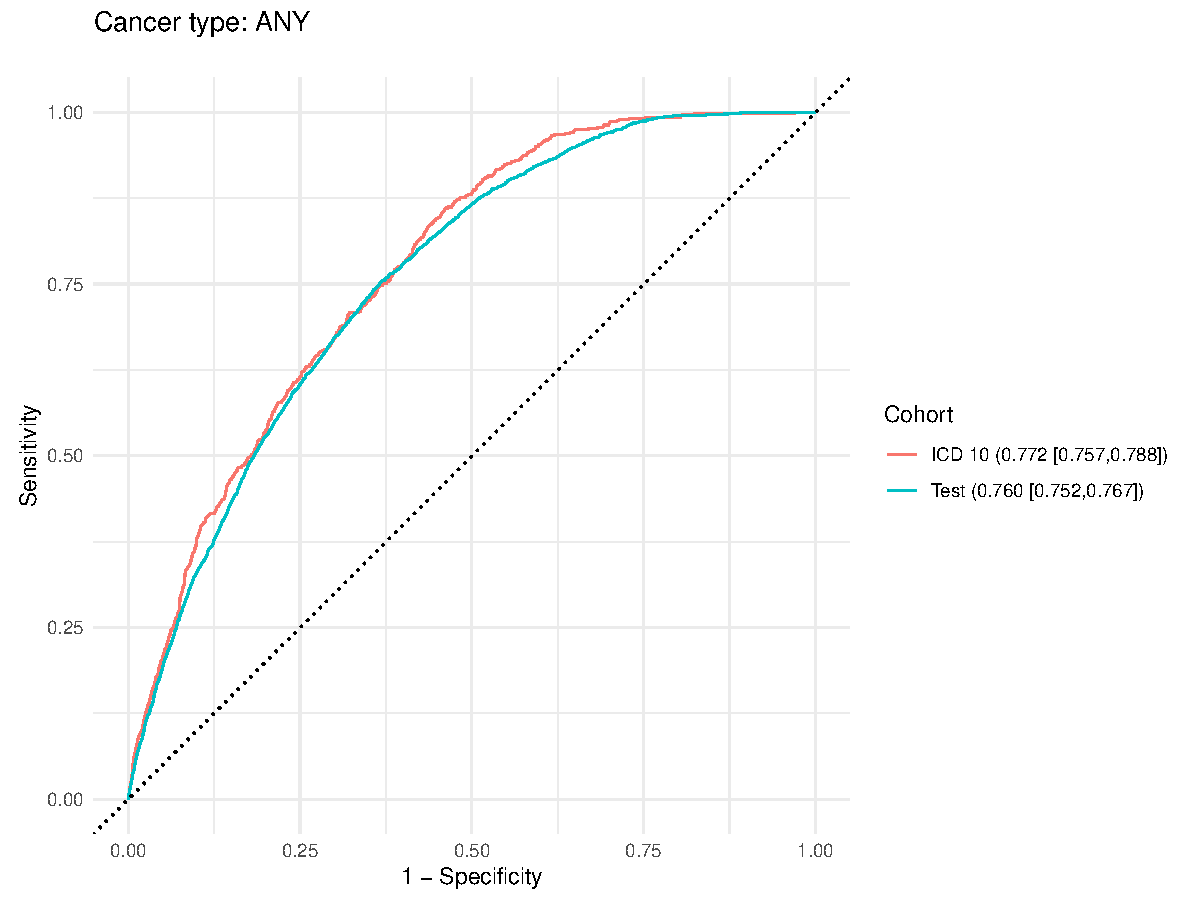
\includegraphics[width=0.8\linewidth]{icd10/roc_ANY.pdf}
\end{figure}
\begin{figure}[h]
\centering
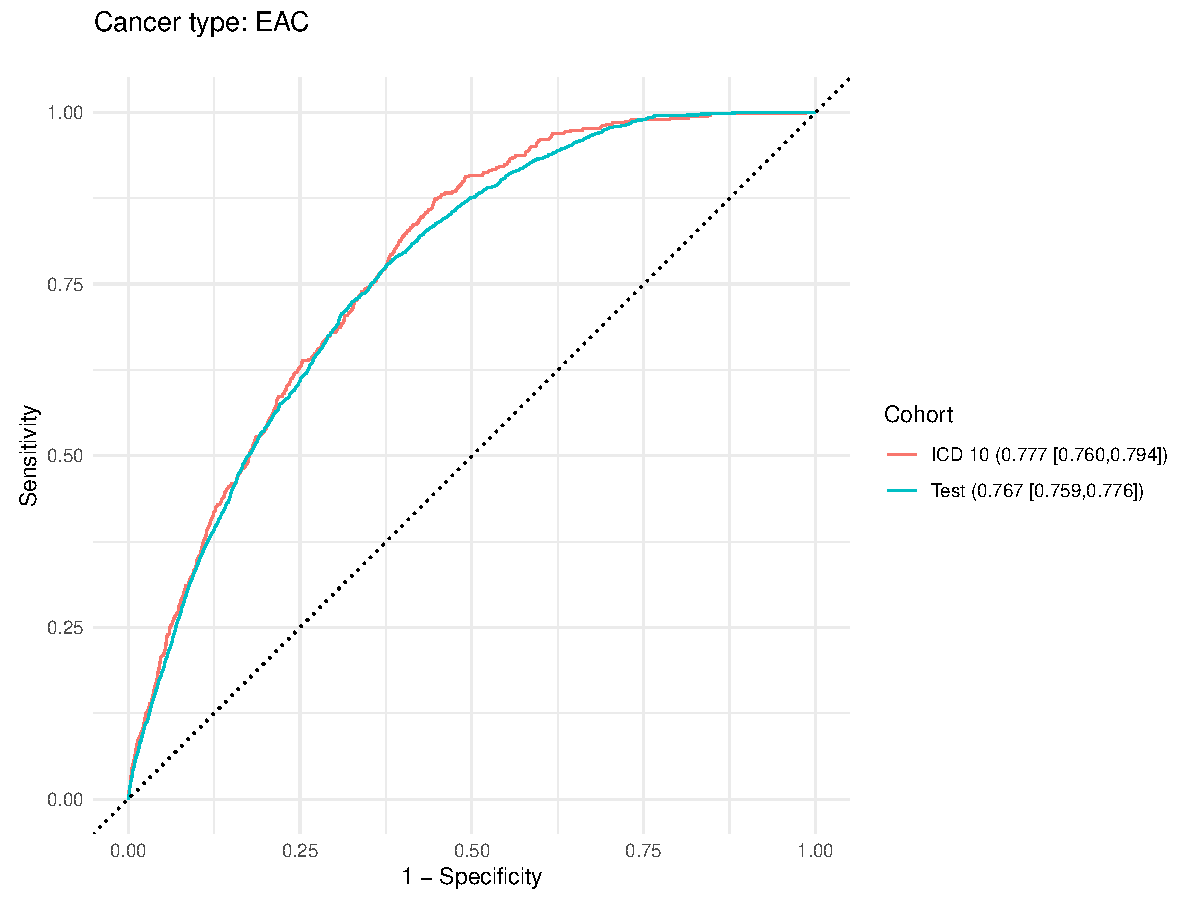
\includegraphics[width=0.8\linewidth]{icd10/roc_EAC.pdf}
\end{figure}
\begin{figure}[h]
\centering
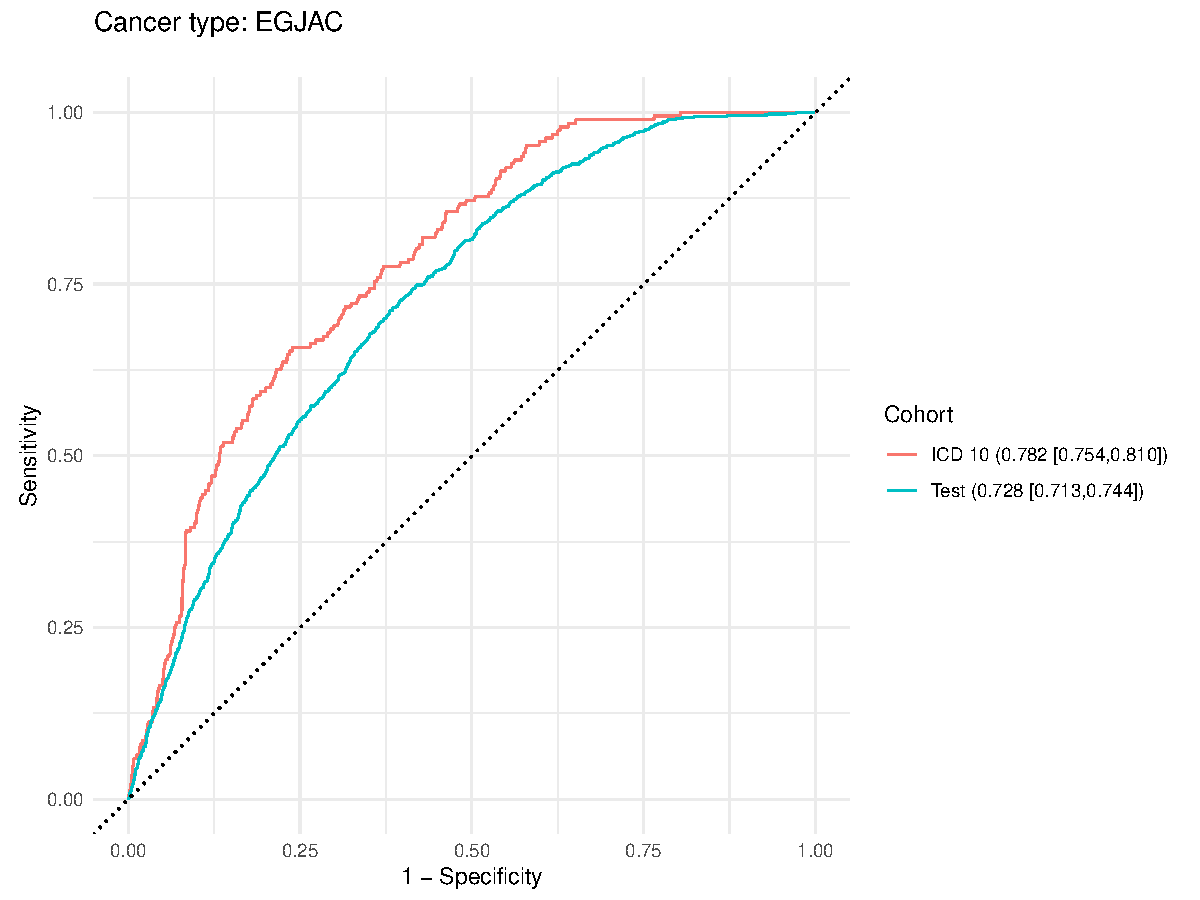
\includegraphics[width=0.8\linewidth]{icd10/roc_EGJAC.pdf}
\end{figure}



\newpage
\clearpage
\section{Discriminative performance comparison on a representative sample}

Comments
\begin{itemize}
	\item Subsample men to 1:1 ratio (not adjusting to case incidence)
	\item All AUCs are increased as was previosuly observed for representative samples
	\item Similar comparison as above
\end{itemize}

\begin{figure}[h]
\centering
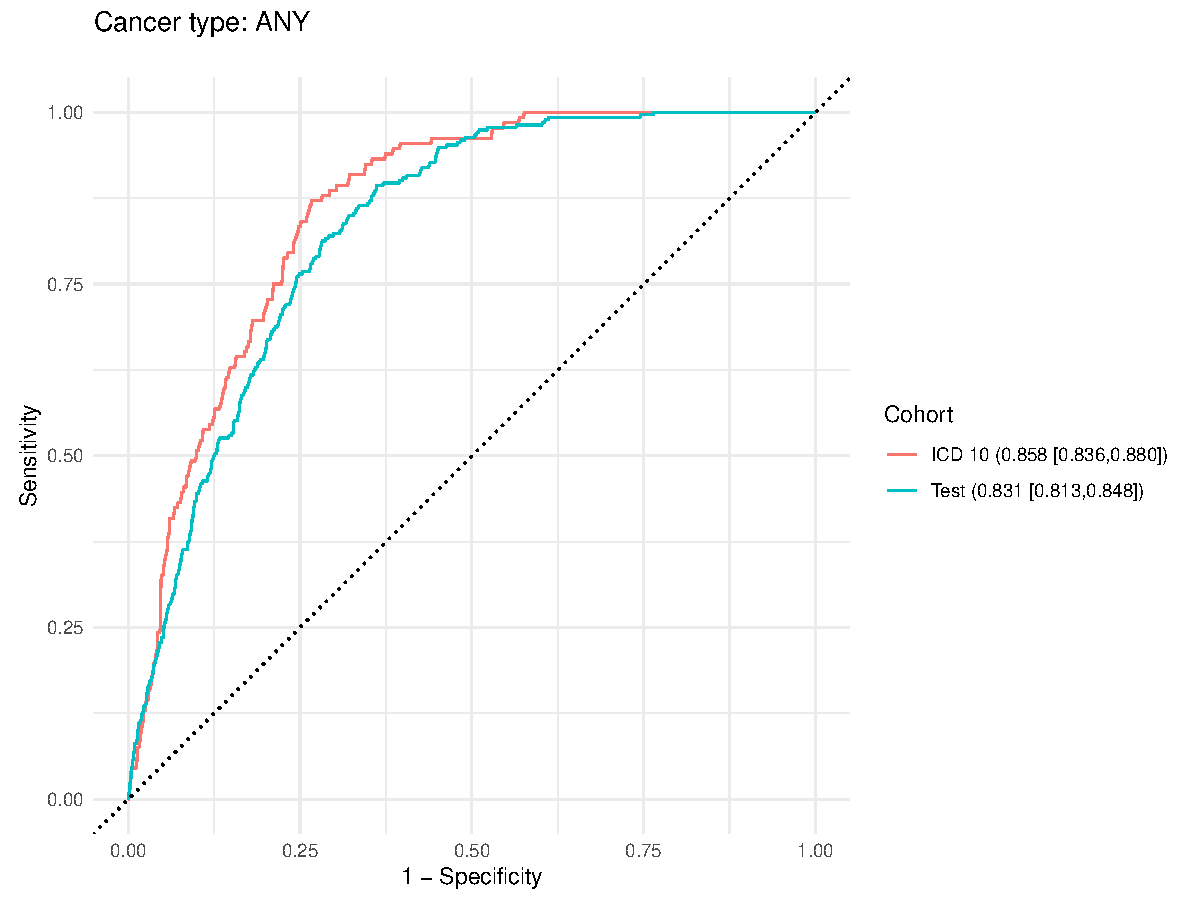
\includegraphics[width=0.8\linewidth]{icd10/roc_ANY_representative.pdf}
\end{figure}
\begin{figure}[h]
\centering
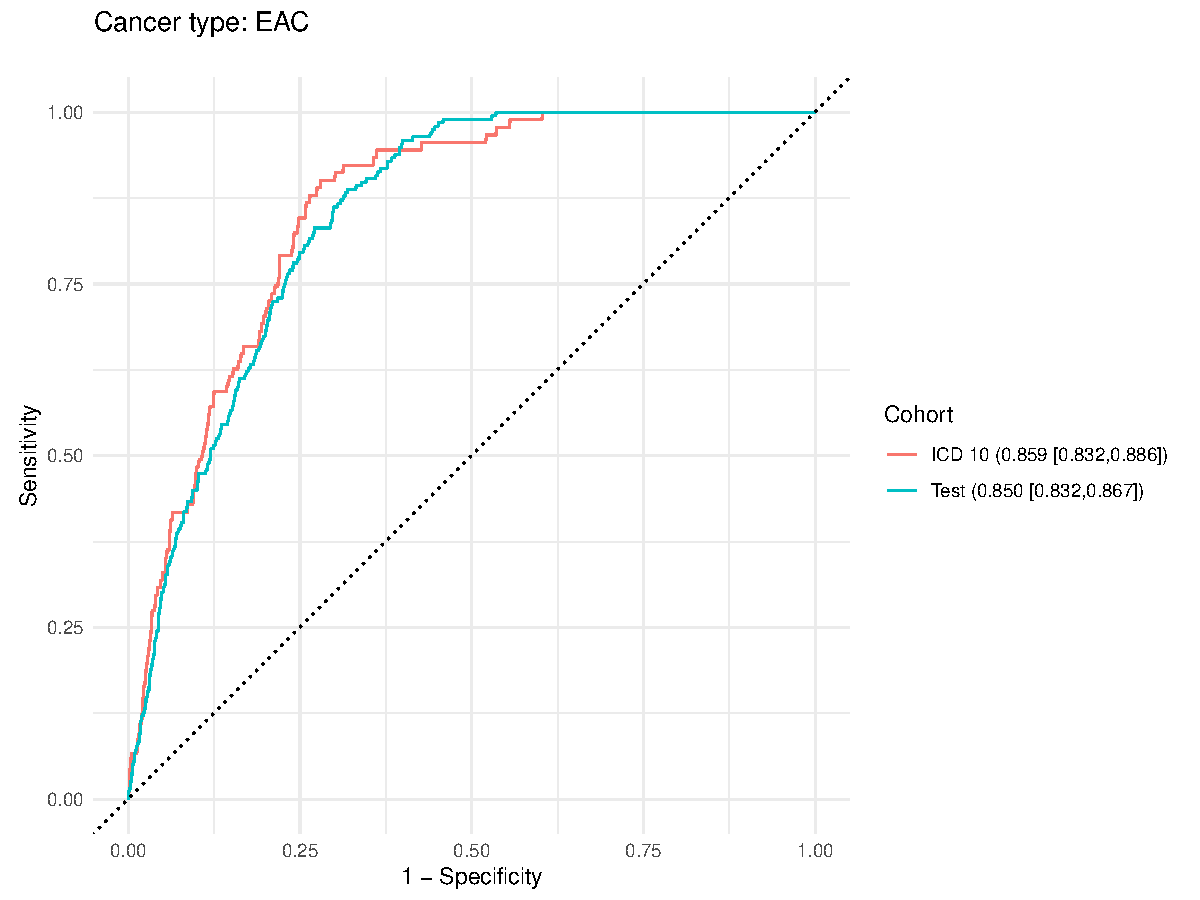
\includegraphics[width=0.8\linewidth]{icd10/roc_EAC_representative.pdf}
\end{figure}
\begin{figure}[h]
\centering
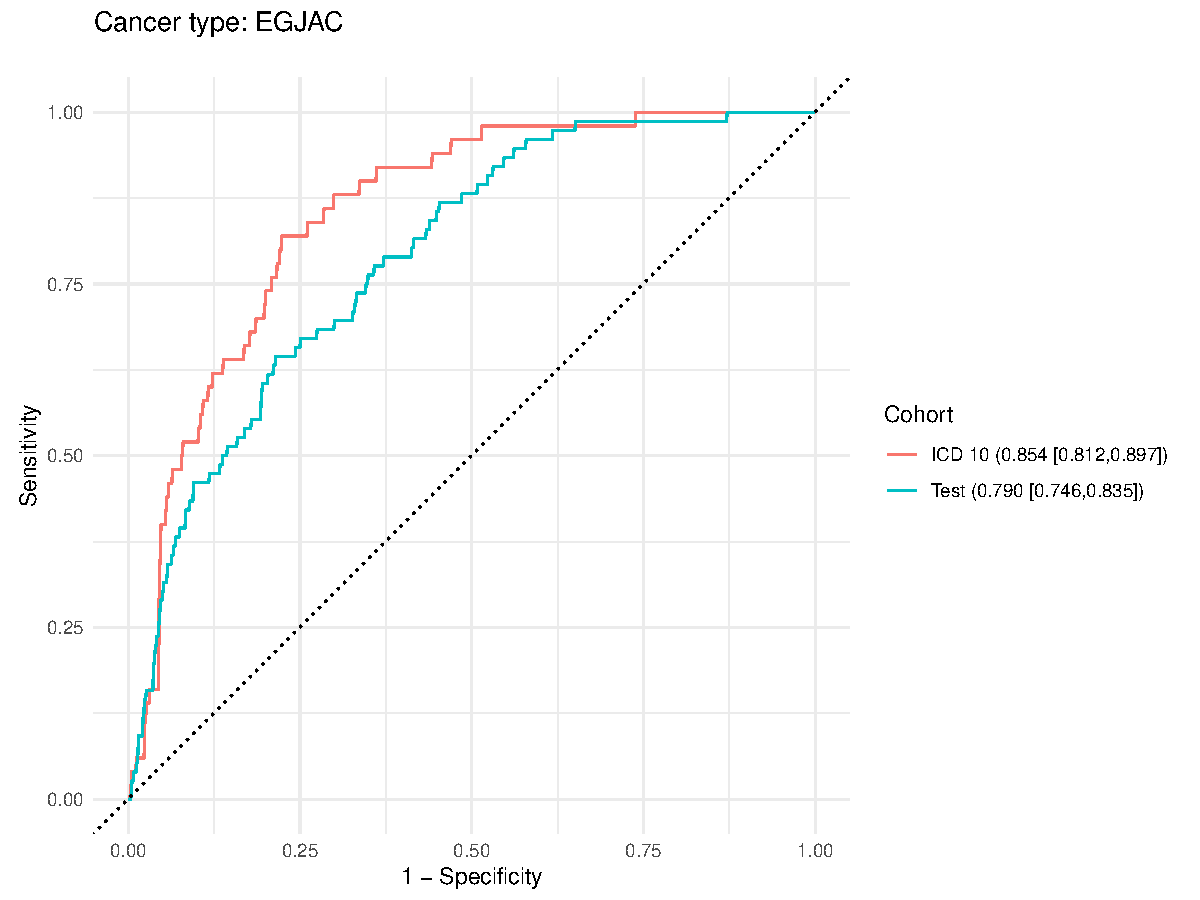
\includegraphics[width=0.8\linewidth]{icd10/roc_EGJAC_representative.pdf}
\end{figure}


\newpage
\clearpage
\section{Risk distribution comparison}

Comments
\begin{itemize}
	\item All three show the exact same trend:
	\item Same two peaks, but the higher risk peak is smaller for ICD 10
	\item Possibly due to the distributional shift; i.e., fewer high-risk patients 
	(fewer men, younger on average)
\end{itemize}

\begin{figure}[h]
\centering
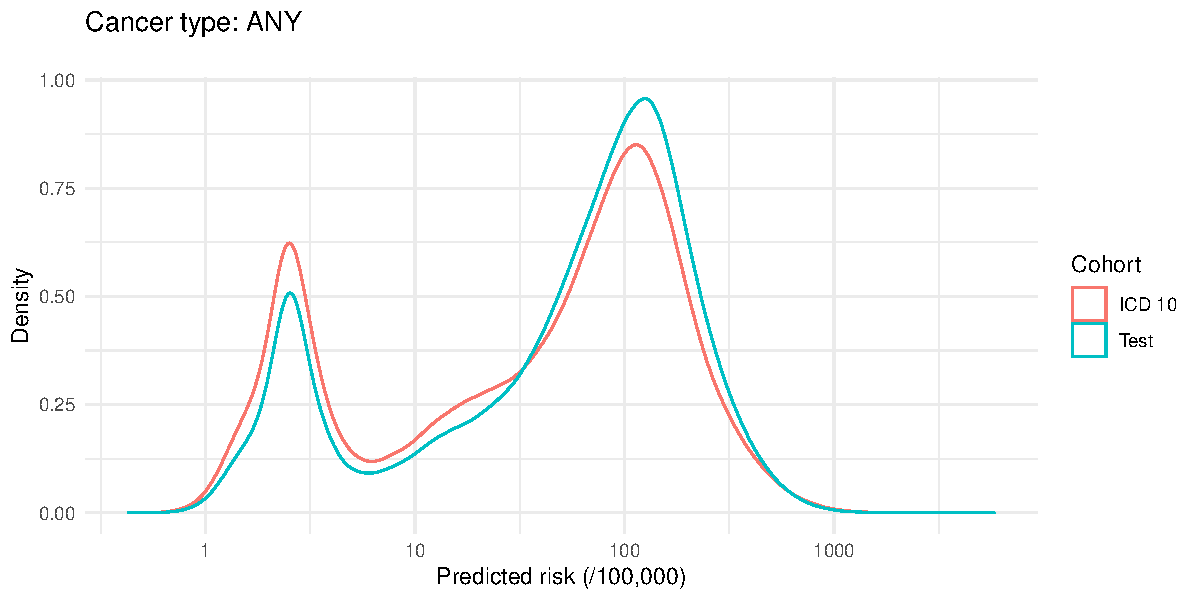
\includegraphics[width=\linewidth]{icd10/score_dist_ANY.pdf}
\end{figure}
\begin{figure}[h]
\centering
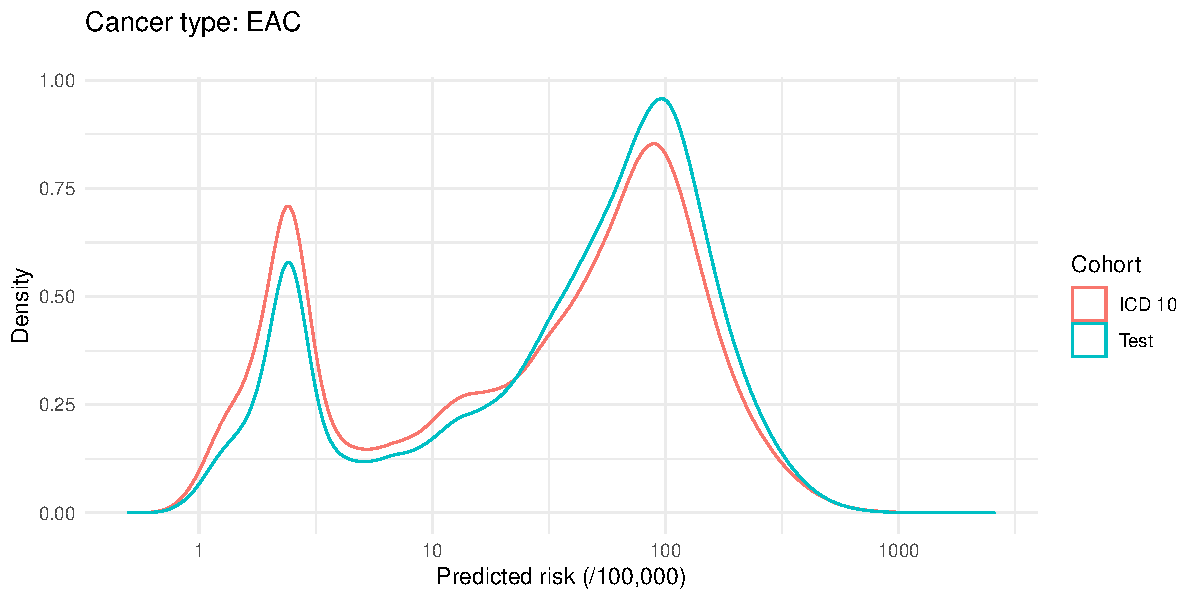
\includegraphics[width=\linewidth]{icd10/score_dist_EAC.pdf}
\end{figure}
\begin{figure}[h]
\centering
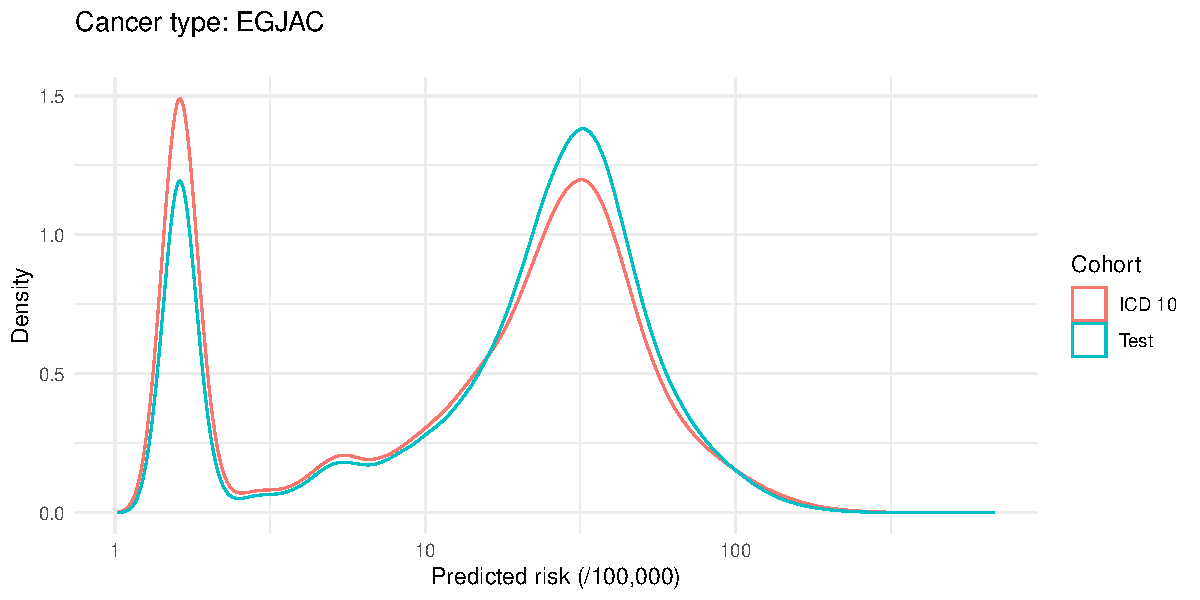
\includegraphics[width=\linewidth]{icd10/score_dist_EGJAC.pdf}
\end{figure}


\newpage
\clearpage

To understand the disparity better, we stratify by age and sex:
\begin{table}[h]
\centering
\begin{tabular}{lrrr}
\toprule
 & \multicolumn{2}{c}{\textbf{Sex}} & \\ \cmidrule{2-3}
 \textbf{Cohort} & Female & Male & \textbf{Ratio M:F} \\
\midrule
\multicolumn{4}{l}{\textbf{Age 0-35}} \\ \addlinespace
  ICD 10 &  89844  &  311775  &  3.5:1\\
  Test   & 64313 & 268890 &   4.2:1\\
\midrule
\multicolumn{4}{l}{\textbf{Age 35-50}} \\ \addlinespace
  ICD 10&  96179 & 344122 &   3.6:1\\
  Test  &  63560 & 311452   & 4.9:1\\
\midrule
\multicolumn{4}{l}{\textbf{Age 50-100}} \\ \addlinespace
  ICD 10 & 154829 &1457904  &  9.4:1\\
  Test   & 86699  &1772155 &   20.5:1\\
\bottomrule
\end{tabular}
\\

\begin{tabular}{lrr}
\toprule
\multicolumn{3}{l}{\textbf{Average age}} \\
 & \multicolumn{2}{c}{\textbf{Sex}} \\ \cmidrule{2-3}
 \textbf{Cohort} & Male & Female \\
\midrule
  ICD 10 &  58.7  &  47.9  \\
  Test   & 60.8 & 46.2\\
\bottomrule
\end{tabular}
\end{table}

Some observations:
\begin{itemize}
	\item Females increased their average age; males decreased 
	\item The biggest shift in proportion of females in the older patients (say, >50 yo)
	\item Females have an increase in the second ``bump''; Males rather have a decrease.
	This seem to match with the change in ratios: the largest change in ratios is in the
	older, more at risk, patients
	\item Stratifying by age seem to completely remove the change in risk distribution. Thus,
	the conclusion seems to be that the shift in risk distribution is mostly explained by
	the shift in age: in particular, since males are by far the most frequent, the decrease 
	in average in men explains most of the shift, even though females have the opposite effect
\end{itemize}

\begin{figure}[h]
\centering
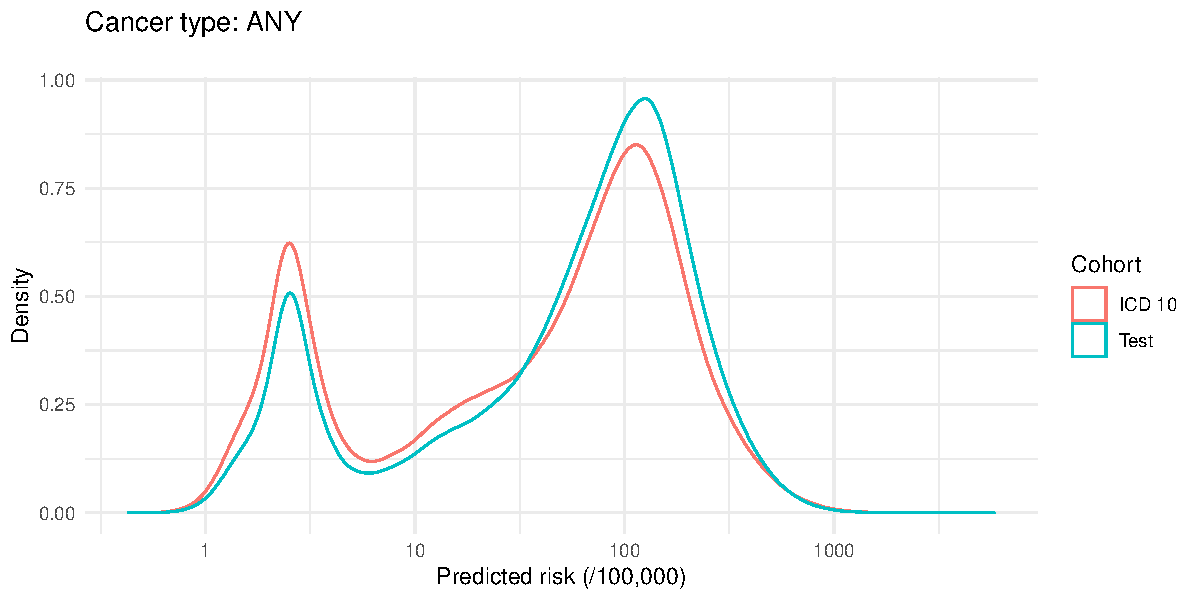
\includegraphics[width=\linewidth]{icd10/score_dist_ANY.pdf}
\end{figure}
\begin{figure}[h]
\centering
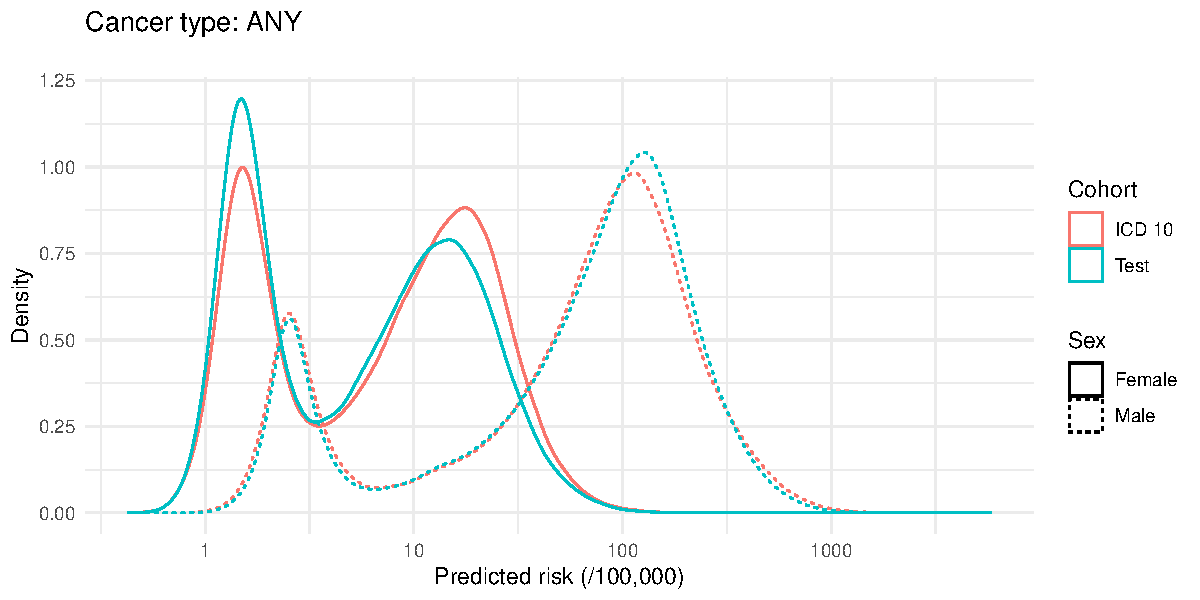
\includegraphics[width=\linewidth]{icd10/score_dist_ANY_bysex.pdf}
\end{figure}
\begin{figure}[h]
\centering
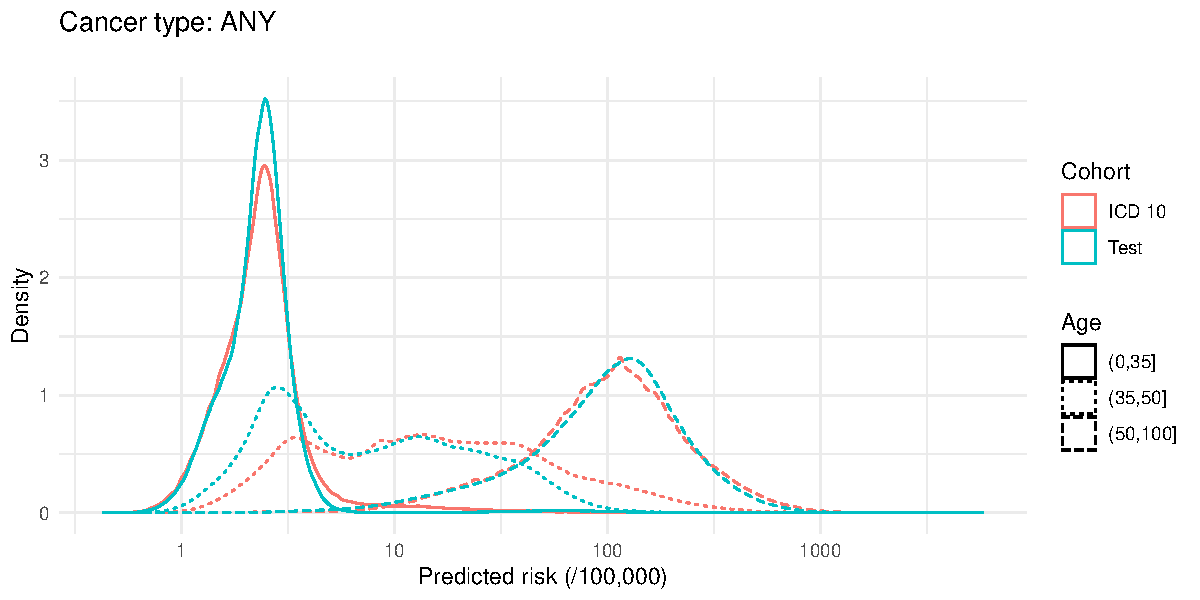
\includegraphics[width=\linewidth]{icd10/score_dist_ANY_byage.pdf}
\end{figure}

\end{document}
